\section{Requisitos}

En esta sección se abordarán los requisitos planteados en la aplicación, tanto los iniciales como los que se han ido planteando a lo largo del desarrollo ya sean funcionales o no funcionales. 

\subsection{Requisitos Funcionales}
\begin{itemize}
    \item RF1. Como usuario puedo rellenar mi nombre, edad y género.
    \item RF2. Como usuario puedo interactuar con las burbujas de cada bioma.
    \item RF3. Como usuario puedo informarme acerca de los alteraciones y problemas de los biomas desde el libro informativo.
    \item RF4. Como usuario puedo relacionar problemas con consequencias y ser informado de si una relación es correcta.
    \item RF5. Como usuario puedo pasar de la fase de investigación a la fase de restauración.
    \item RF6. Como usuario puedo ver en la tienda distintas máquinas restauradoras con distinos efectos.
    \item RF7. Como usuario puedo colocar una máquina y ver que tiene efecto sobre el bioma.
    \item RF8. Como usuario puedo vender esa máquina si opino que no ha funcionado como esperaba.
    \item RF9. Como usuario puedo reiniciar una fase si una máquina destruye el ecosistema.
    \item RF10. Como usuario puedo reiniciar un nivel si me quedo sin dinero u opino que he cometido un error crítico.
    \item RF11. Como usuario puedo abrir el libro informativo en cualquier momento para consultar la información y relaciones de los problemas.
    \item RF12. Como usuario puedo ver el progreso actual de cada fase de cada bioma.
    \item RF13. Como usuario puedo terminar una fase colocando suficientes máquinas restauradoras correctamente.
    \item RF14. Como usuario puedo terminar un nivel una vez he terminado todas las fases de todos los biomas.
\end{itemize}

\subsection{Requisitos No Funcionales}

\begin{itemize}
    \item RNF1. El videojuego tiene que ser divertido.
    \item RNF2. El videojuego tiene que tener una usabilidad mínima.
    \item RNF3. El videojuego debe ser divulgativo en lo referente al a restauración de ecosistemas.
    \item RNF4. El videojuego debe desarrollar el PC
    \item RNF5. El videojuego debe tener herramientas que ayuden al desarrollo de contenido
    \item RNF6. El videojuego debe ser multiplataforma (PC, Tablet, Móvil, Web).
\end{itemize}

\subsection{Requisitos de Diseño}

\begin{itemize}
    \item RD1. Cada nivel del videojuego debe tener 1-N biomas posibles.
    \item RD2. Cada bioma debe tener dos alteraciones posibles.
    \item RD3. Al iniciar el nivel, se deberá elegir una alteración de las dos posibles por cada bioma.
    \item RD4. Cada alteración deberá tener 1-3 problemas relacionadas (Figura \ref{fig:diagramaalt}).
    \item RD5. Cada problema deberá tener de 0-2 problemas y de 1-4 consecuencias relacionados.
    \item RD6. Cada problema deberá tener 2-3 máquinas relacionadas.
\end{itemize}

\begin{figure}[H]
    \centering
      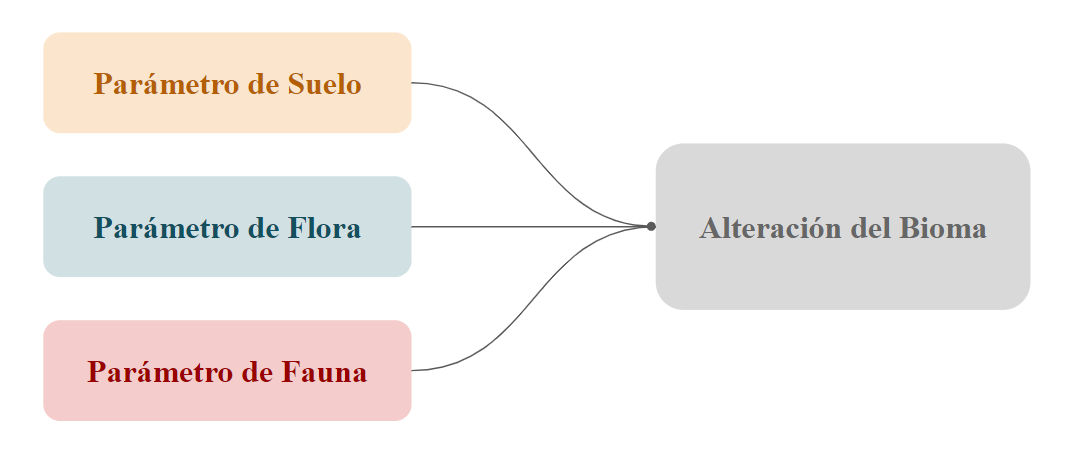
\includegraphics[width=350px,clip=true]{diagramaalteracionproblemas.png}
    \caption{Diagrama que muestra la relación entre problemas y alteraciones}
    \label{fig:diagramaalt}
\end{figure}

\section{Herramientas y Tecnologías}

\subsection{C\# \& Unity}

Se ha utilizado Unity\cite{unity} como motor para el desarrollo de EcoRescue y C\#\cite{csharp} como lenguaje de programación, se ha elegido este motor dado que era el motor público con el que los desarrolladores teníamos más experiencia.

\subsection{Visual Studio}

Visual Studio\cite{visualstudio} es un IDE y editor de código para C++ y .Net y C\#, es el editor de código por defecto de Unity y el que se ha utilizado por defecto para el desarrollo del proyecto. 

\subsection{Git \& Github}

Github\cite{github} es un entorno de desarrollo colaborativo y control de versiones web basado en la tecnología Git. Para mantener el proyecto y poder trabajar en el desde distintos equipos, se ha alojado el proyecto de EcoRescue\cite{Repo} en él.

\subsection{FastNoiseLite}

La generación procedimental de los mapas de los niveles del prototipo utilizan texturas de ruido perlin generadas automáticamente por la librería FastNoiseLite\cite{FastNoiseLite}. Esta es una librería ligera, optimizada y muy sencilla de usar que permite obtener patrones aleatorios altamente personalizables de una forma muy cómoda y sencilla.

\subsection{Adobe XD \& AkyuiUnity}

Adobe XD\cite{xd} es un programa que forma parte de la 'Suite' creativa de Adobe, permite a los usuarios el desarrollo de interfaces basado en iconos y formas vectoriales. \nombrecoautorespacio ha utilizado este programa para desarrollar las interfaces e iconos del videojuego. Esta herramientas se ha aprovechado enormemente mediante el uso de AkyuiUnity\cite{AkyuiUnity} y AnKuchen\cite{AnKuchen}, dado que el conjunto de estas dos librerías permiten establecer un flujo de trabajo mediante el cual se pueden importar los proyectos de Adobe XD como prefabs dentro de Unity, además de auto generar clases para poder acceder a todos los elementos del prefab a partir de su ID. Este 'workflow' ha permitido que el desarrollo e implementación de interfaces sea muy dinámico y fluido. 

\subsection{UniTask}

UniTask\cite{UniTask} es una librería que ofrece una implementación de async/await sin necesidad de alocataciones de memoria basada en estructuras. Se ha aprovechado esta librería para la implementación de varias rutinas de comportamiento del prototipo, desde eventos de UI hasta los propios controles del juego.

\subsection{DUJAL}

DUJAL\cite{DUJAL} es una librería de creación propia para otro Trabajo de Fin de Grado, esta librería contiene utilidades como un sistema de diálogos basado en grafos, un sistema de sonido estático y accesible desde todo el proyecto, llamadas estáticas a sacudidas de cámara, controladores de personajes y más. En este proyecto se ha importado solamente los módulos de diálogo, sonido y guardado de partida.

\subsection{Audacity}

Audacity\cite{Audacity} es un programa de edición y grabación de audio, todos los sonidos del videojuego se han obtenido retocando samples de uso libre utilizando Audacity.  

\subsection{Notion}

Notion\cite{notion} es una plataforma para la creación de documentos, wikis, listas de tareas y más. Para el desarrollo del proyecto se ha utilizado Notion como base de la documentación para almacenar toda la información referente al diseño, implementación, contenido y referencias artisticas y mecánicas.

\subsection{MariaDB \& SQL}

Para el almacenamiento de datos acerca de los jugadores y las partidas, se ha utilizado una base de datos proporcionada por la URJC basada en MariaDB\cite{mariadb}, un modelo de base de datos relacional que sigue el estándar SQL.


\section{Arquitectura y Análisis}
\subsection{Clases 'Handler' y diseño con enumerados}
EcoRescue está implementado de forma que todo el juego se pueda gestionar a partir de clases de tipo 'Singleton' que contienen referencias a tipos de datos que contienen el estado actualizado de la partida. Estos managers estáticos se encargan de gestionar una parte concreta del juego y sus funciones relacionadas.

Para entender cómo funcionan estas clases gestoras, primero hay que explicar el patrón de diseño que se ha utilizado de cara a organizar el gran volumen de datos necesario para hacer un juego de este tipo de forma procedimental. Este patrón consiste en utilizar enumeraciones para identificar inequívocamente a un 'ScriptableObject' que representa un elemento de juego, para el ejemplo podemos utilizar una 'Machine'. Una 'Machine' tendrá asociado un 'MachineType' que deberá ser único para este 'ScriptableObject' en particular. De esta forma, cuando se esté tratando esta máquina y no se necesite acceder a nada que no sea su nombre, se puede utilizar este enumerado para identificarla. 

Este patrón satisface dos problemas a resolver, el primero es poder utilizar el nombre del enumerado como string en un archivo de tipo excel de cara a poder autogenerar los enumerados de C\#, de forma que el contenido se importe automáticamente mediante un MenuItem de Unity, el segundo motivo es que permite ahorrar memoria a la hora de crear estructuras que necesiten contener listas de ScriptableObject, dado que se estaría guardando únicamente el valor del enumerado, en lugar de tener que hacer copias del propio archivo del ScriptableObject para poder utilizar los valores. Para acceder a los valores que contiene el 'ScriptableObject' se almacena en la clase gestora un diccionario que relaciona el valor del enumerado con el 'ScriptableObject' almacenado en memoria. 

\subsection{Biome, Machine, Relation y Phase 'Handlers'}

Estas clases (Figura \ref{fig:handlerUML}) utilizan todas el patrón mencionado anteriormente, 'BiomeHandler' y 'MachineHandler' tienen diccionarios que contienen relaciones entre Biomas y Máquinas con sus respectivos enumerados, además de una lista de todos los enumerados posibles para el nivel actual. 'RelationHandler' es ligeramente más compleja en el sentido de que tiene tres sets de listas y diccionarios, para alteraciones, problemas y consecuencias. Todas estas clases se poblan en base a los datos que se reciben del nivel seleccionado (contenido en el 'ScriptableObject' de la clase 'Level'). De forma que en todo momomento contienen la información actualizada del nivel actual, que puede ser consultada por la lógica del juego cuando es requerida. 

Cabe destacar que cada una tiene funciones especializadas, ya sea el 'MachineHandler' para guardar información de un diccionario que relacione las máquinas colocadas en el tablero de juego con la casilla sobre la que se encuentran colocadas en ese momento. O BiomeHandler, que relaciona cada bioma con todas las casillas asociadas a este.
  
\begin{figure}[H]
    \centering
      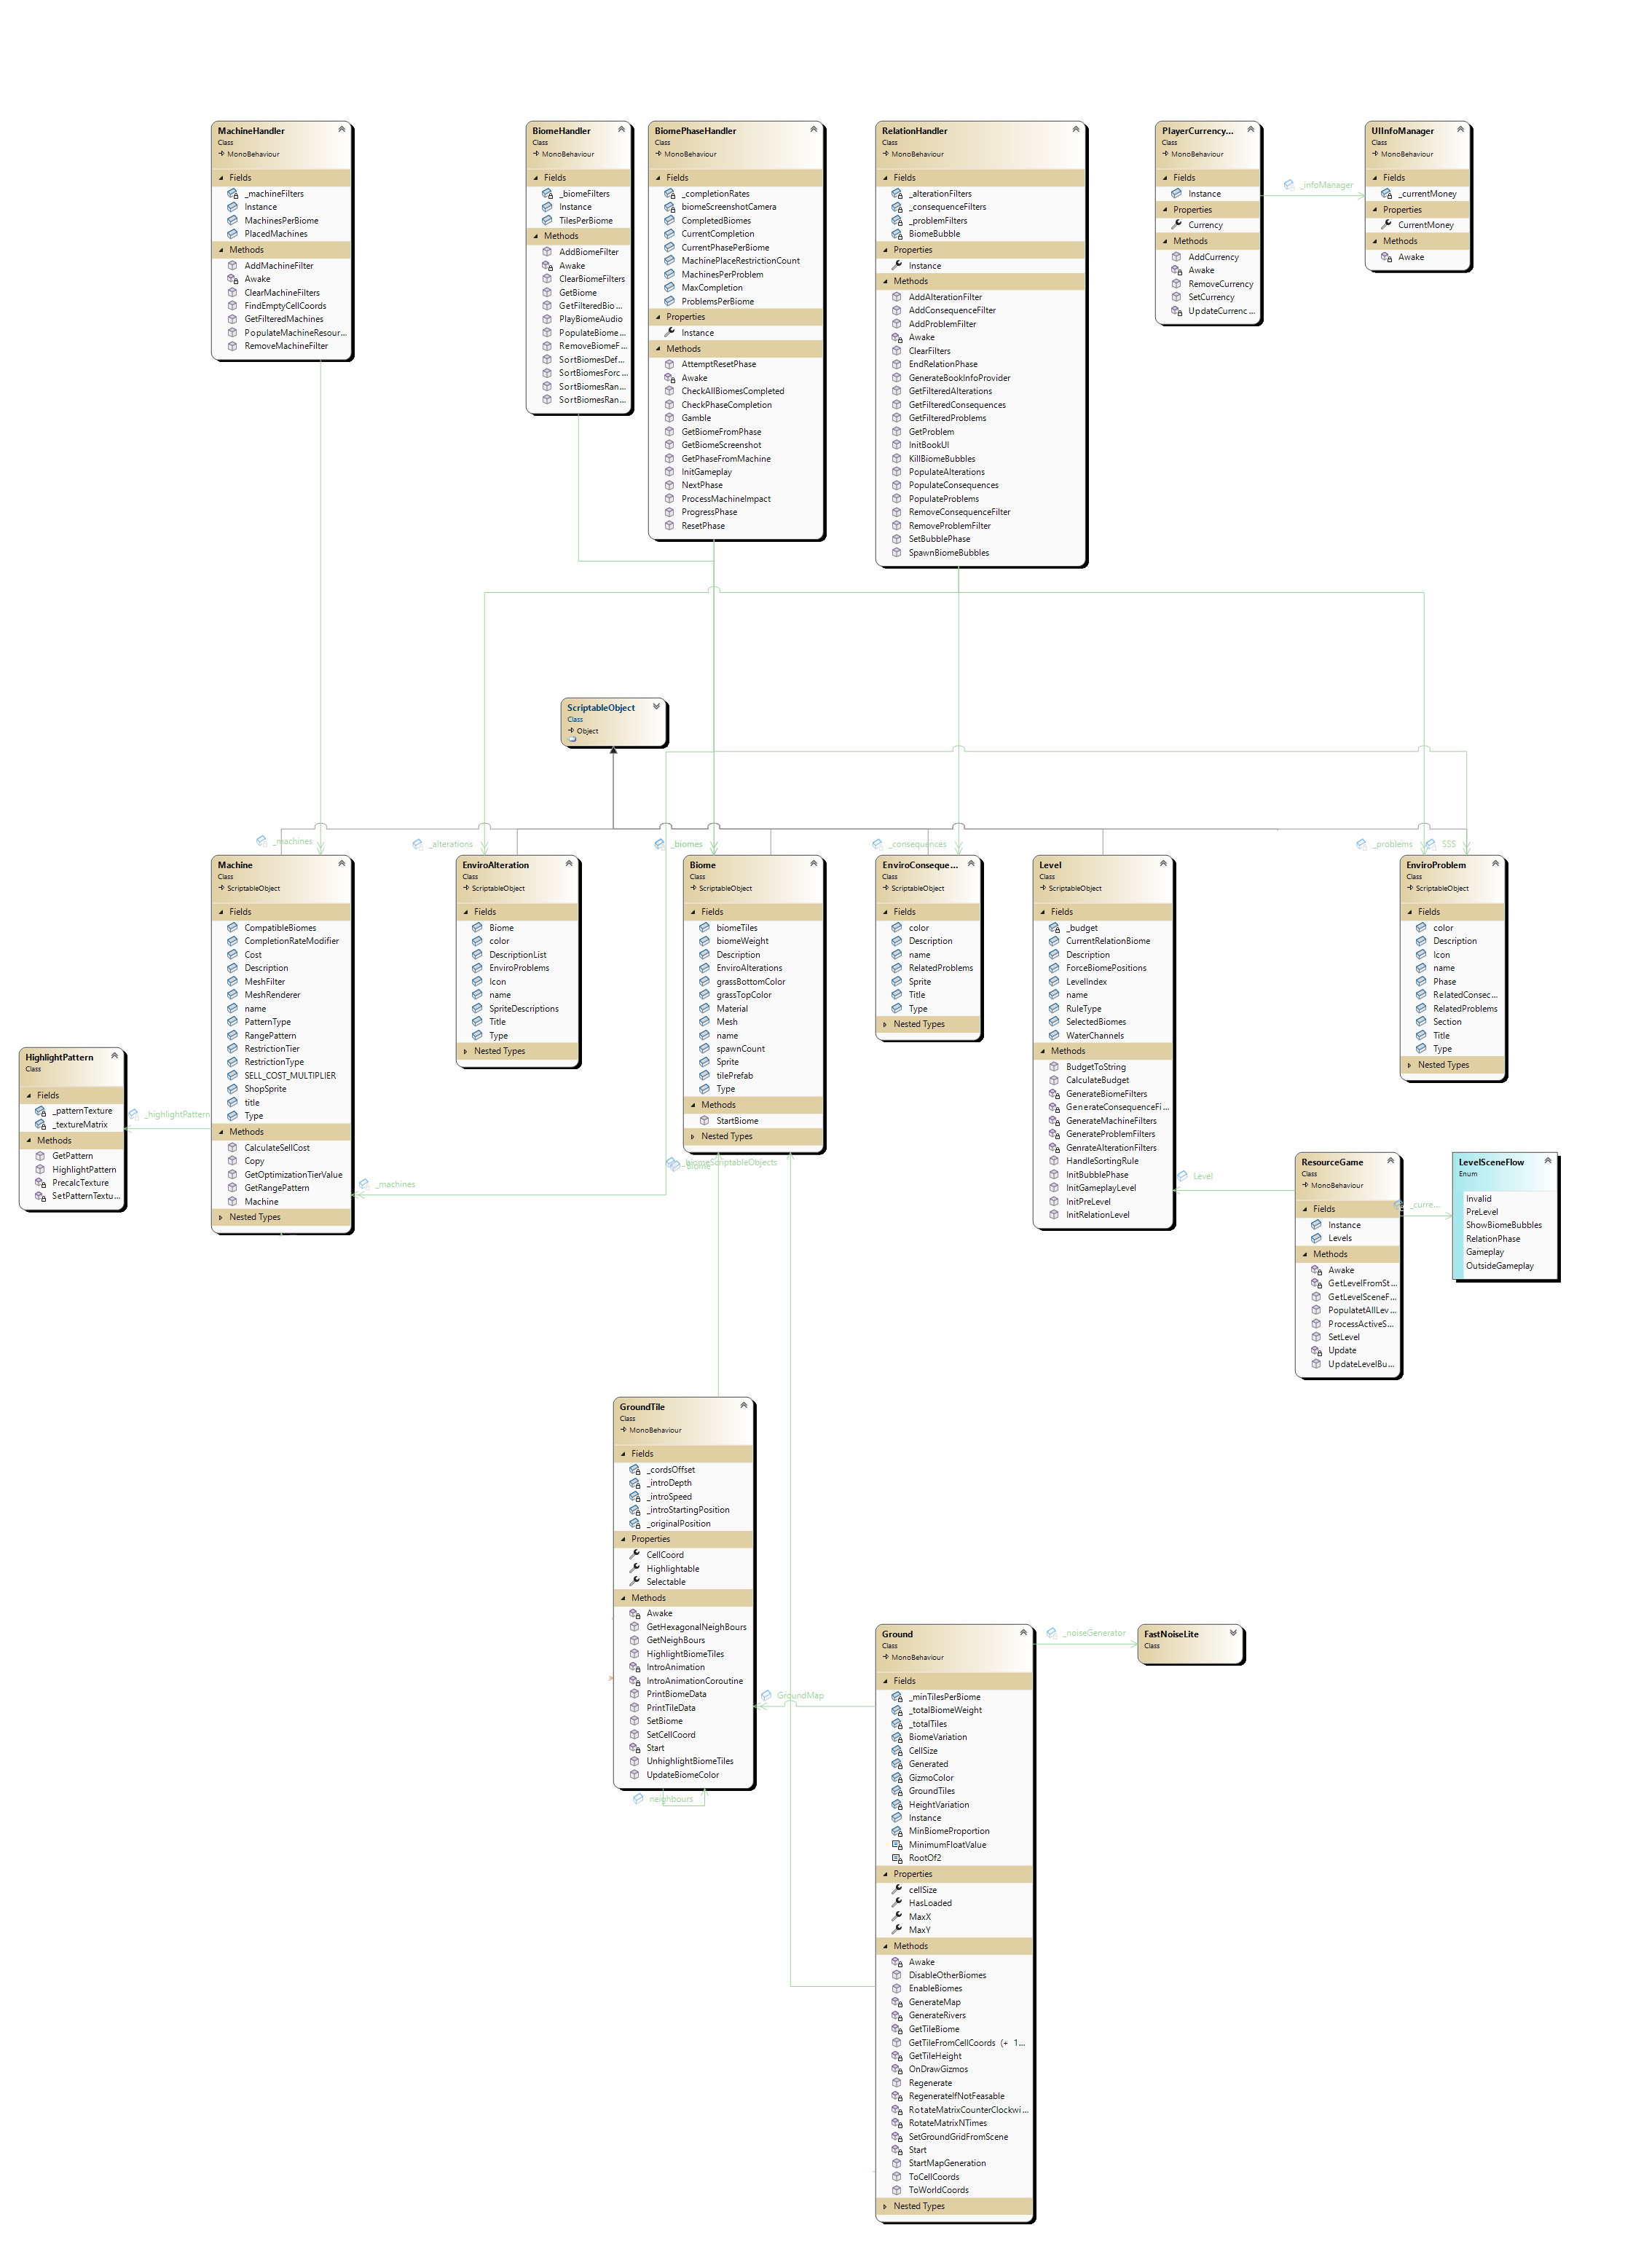
\includegraphics[width=350px,clip=true]{Handler_Class_Diagram.png}
    \caption{Diagrama de clases de los Handlers y ResourceGame}
    \label{fig:handlerUML}
\end{figure}


Por último, el 'BiomePhaseHandler' es el que se encarga de gestionar toda la progresión de la fase de restauración, contiene diccionarios que relacionan todos los problemas que hay en el nivel actual por cada bioma y todas las máquinas posibles por cada problema. Además de diccionarios que relacionan el percentil (Figura \ref{fig:progresion}) mínimo de compleción por fase, la compleción actual por fase o la fase actual por bioma. Esta clase se encarga de registrar si al colocar una máquina esta restaura correctamente el problema relacionado o si en su lugar destruye el ecosistema y fuerza el reinicio de esa fase en ese bioma, y también se encarga de comprobar cuándo se pasa de fase así como de comprobar si todas las fases se han completado.

\begin{figure}[H]
    \centering
      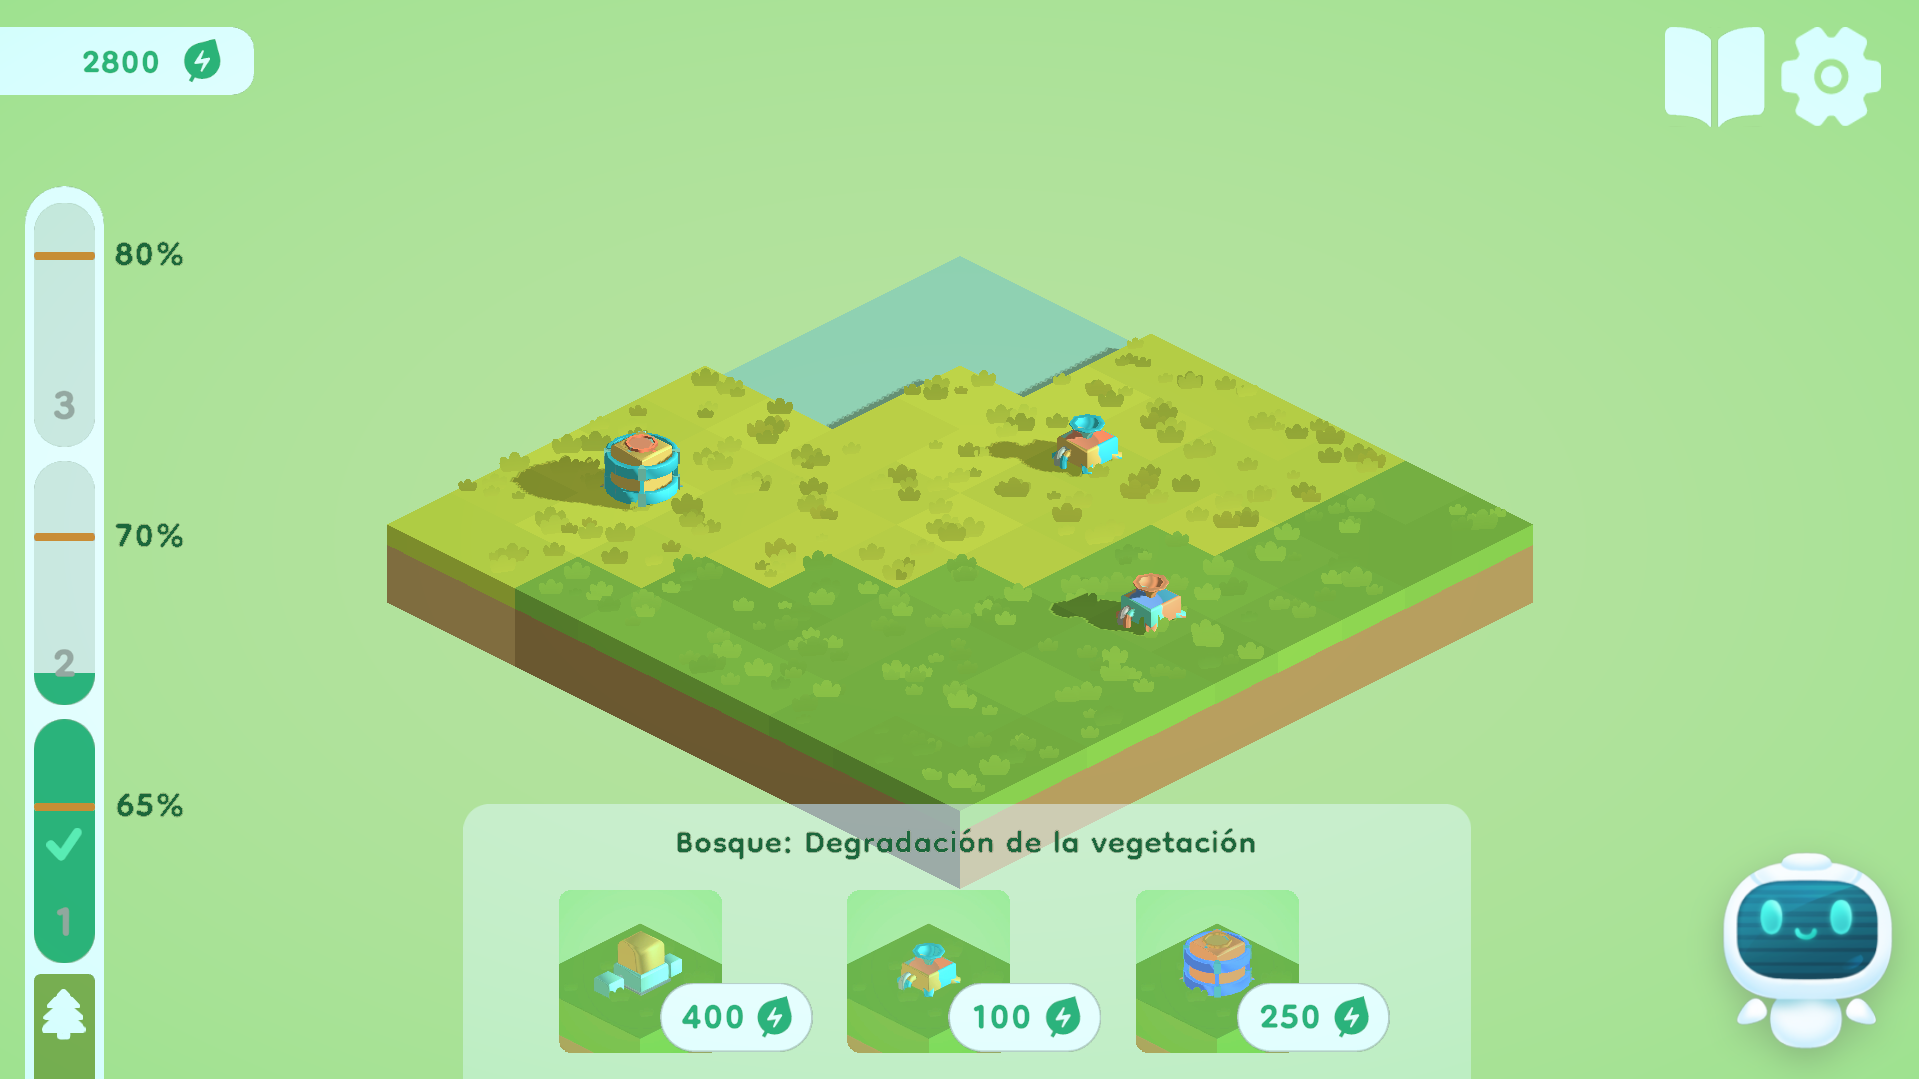
\includegraphics[width=350px,clip=true]{progresion.png}
    \caption{Interfaz de progresion de la fase de restauración}
    \label{fig:progresion}
  \end{figure}

\subsection{ResourceGame y Level}

'ResourceGame' es la clase que gestiona las fases y los datos de un nivel, este lee todos los niveles que existan dentro de la carpeta de 'Levels' y carga el que el botón del selector de niveles le pase por argumento.

La clase 'Level', por otro lado, contiene las funciones que poblan todos los 'Handlers', y que gestionan el flujo de un nivel.
\begin{itemize}
    \item InitPreLevel - 'Cachea' todos los datos del Level en las estructuras de datos contenidas en los 'Handlers'.
    \item InitBubblePhase - Instancia las burbujas que abren el libro de relaciones encima de cada bioma.
    \item InitRelationLevel - Inicializa el libro de relaciones y espera a que se hayan completado todas las relaciones de todos los biomas.
    \item InitGameplayLevel - Habilita la tienda y pasa al modo colocar máquinas, se queda así hasta que se restauran todos los ecosistemas.
\end{itemize}

La clase Level también dobla como herramienta de desarrollo, ya que al ser un 'ScriptableObject' permite al diseñador modificar sus propiedades desde el editor. En este caso, se ha añadido una serie de reglas y opciones de personalización que permiten al diseñador elegir qué clase de reglas quiere que la generación procedimental siga. También permite seleccionar qué biomas van a estar presentes en ese nivel. 

\subsection{Ground \& Generación Procedimental}

La clase 'Ground' se encarga de instanciar todas las casillas del mapa siguiendo una serie de reglas definidas en la clase Level. La generación procedimental utiliza una matriz discretizada a partir de un mapa de ruido perlin generado mediante la librería de FastNoiseLite\cite{FastNoiseLite}. La altura del mapa perlin se utiliza para definir qué bioma va en cada lugar, para asegurar que el juego no es injusto se aplican una serie de cupos de casillas mínimas por cada bioma, si el mapa generado no lo cumple, se regenera.

Cada casilla contenida en Ground tiene asignado un componente de tipo GroundTile, con información relevante acerca del bioma y coordenadas discretas de esa casilla en concreto. 

\subsection{PlayerCurrencyManager}

La clase 'PlayerCurrencyManager' es una clase sencilla que solamente se encarga de mantener actualizado el presupuesto de energía del jugador en todo momento. Gestiona las transacciones de compra y venta de máquinas durante la fase de restauración.

\subsection{Interfaces, XD y AnKuchen}

Todas las interfaces del juego se han ilustrado en Adobe XD y convertido en prefabs utilizando AkyuiUnity\cite{AkyuiUnity}, que permite generar prefabs a partir de la definición de formato de interfaz Ankyui desarrollada por kyubuns. Akyui.Xd a su vez permite convertir los archivos en formato de AdobeXD en archivos de definición de formato de Akyui, de forma que se genera un workflow Adobe XD - Unity directo.

Mediante el uso de AnKuchen\cite{AnKuchen}, también desarrollado por kyubuns, se pueden autogenerar unas clases 'template' a partir de las estructuras en el arbol de la escena de Unity mediante el uso de un componente UICache (Figura \ref{UIuml}), estas 'templates' permiten al programador acceder a los elementos de interfaz ('scrollbar', 'button', 'slider') desde código sin necesitar de preocuparse por referencias o jerarquías. Esta librería, en conjunto con UniTask\cite{UniTask} permite definir comportamientod de interfaces de forma muy cómoda.

\begin{figure}[H]
    \centering
      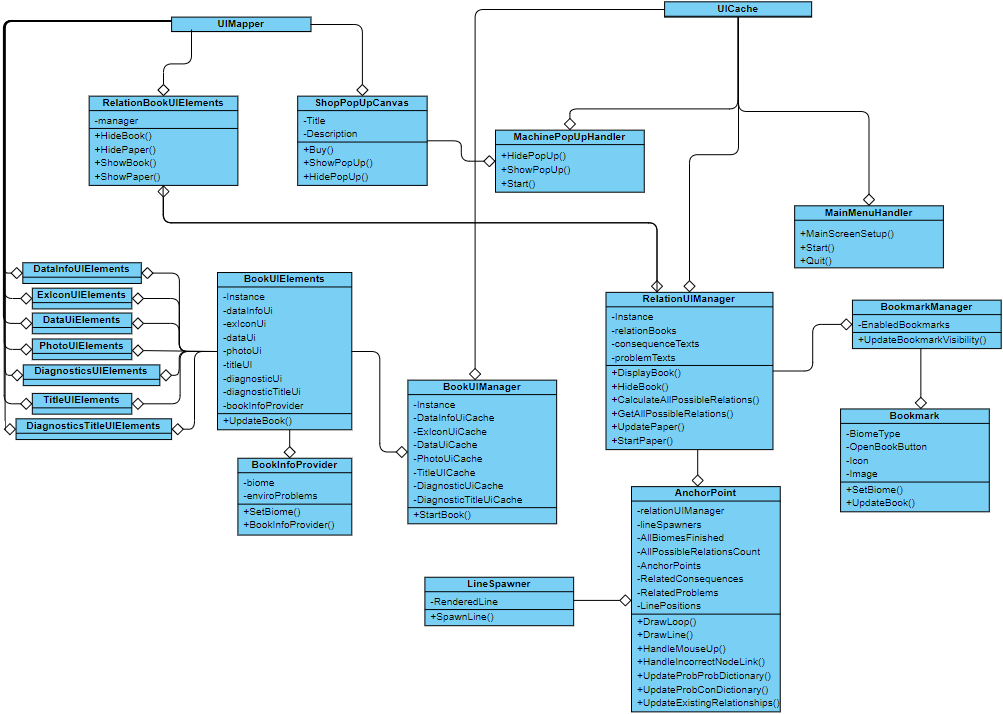
\includegraphics[width=350px,clip=true]{UI_Class_Diagram.png}
    \caption{Diagrama de clases de la UI del juego}
    \label{UIuml}
\end{figure}

\subsection{Cargas, Audio y Diálogos}

EcoRescue utiliza un sistema de carga asíncrona que lanza una pantalla de carga mientras se cargan cosas por detrás, además de un sistema de gestión de audio y una herramienta de creación de diálogos basada en grafos (Figura \ref{fig:dialogue}). Sin embargo estas herramientas son parte de DUJAL\cite{DUJAL} y quedan fuera del alcance de este documento. 

\begin{figure}[H]
    \centering
      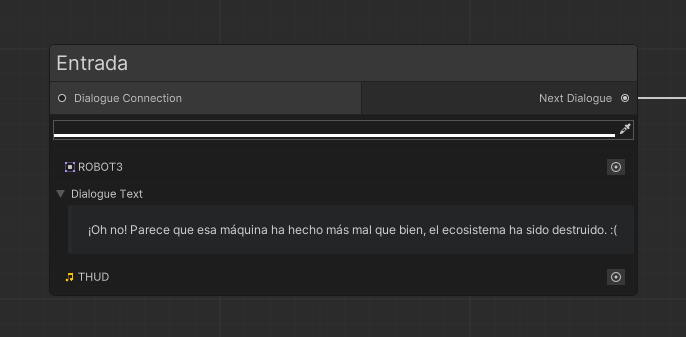
\includegraphics[width=350px,clip=true]{dialogue.png}
    \caption{Herramienta de generación de diálogos}
    \label{fig:dialogue}
\end{figure}

\section{Diseño e Implementación} 

\subsection{Controles}

El componente de control de EcoRescue es una de las partes de la implementación que más tiempo ha llevado, esto es por que el objetivo era que fuese lo más satisfactorio e intuitivo posible. De esta forma, los componentes que gestionan el poder colocar y mover máquinas (Figura \ref{fig:controlUML}) están organizados en jerarquías de herencia que permiten controlar la forma en la que se interactúa con estas de forma modular y sencilla. Las PlaceableMachines, que son las instancias de las máquinas que se pueden colocar, heredan del componente Draggable (Que a su vez hereda de Hoverable). 
\begin{itemize}
    \item Hoverable gestiona el hecho de poder pasar el ratón/dedo por encima de una entidad y lanzar un callback cuando ese evento ocurra. 
    \item Draggable mantiene ese comportamiento, pero también tiene funcionalidad para poder arrastrar el propio GameObject
    \item PlaceableMachine permite invocar la interfaz contextual que se encarga de permitir mover, colocar y vender las máquinas, además de tener una copia profunda del ScriptableObject de la máquina a partir de la cuál se ha creado. 
\end{itemize}

\begin{figure}[H]
    \centering
      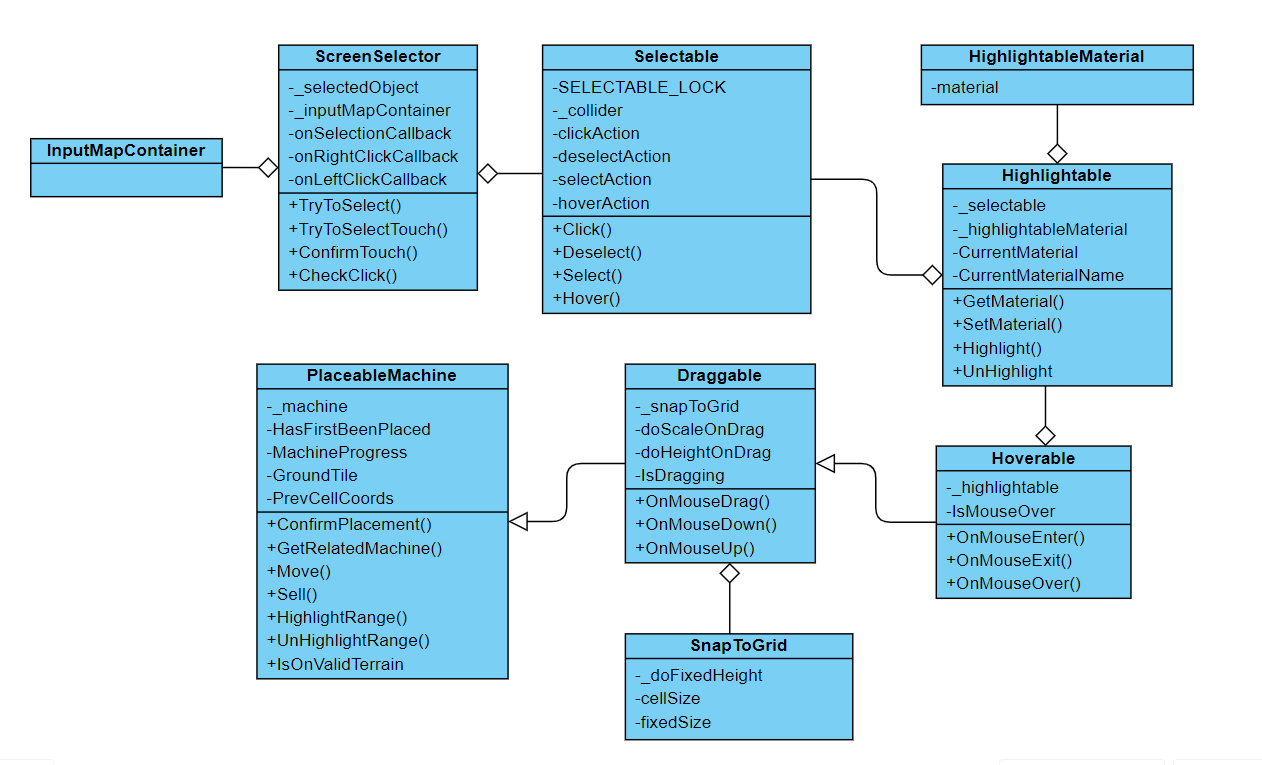
\includegraphics[width=350px,clip=true]{Controls_Class_Diagram.png}
    \caption{Diagrama de clases de las clases de control del juego}
    \label{fig:controlUML}
\end{figure}

Además, para poder añadir comportamiento de resaltado a las casillas y máquinas, se ha añadido un componente de tipo Highlighteable a todos los componentes de tipo Hoverable, de forma que se puede modificar el shader y el material del MeshRenderer utilizando el string asociado al tipo de 'Highlight' que corresponda.

Los componentes de tipo Hoverable, además, tienen una referencia (obligatoria) a un componente Selectable, cuya implementación permite lanzar un callback cuando se interactúe con el ratón o el dedo con dicho Hoverable. Esto permite al componente PlaceableMachine suscribirse al evento de 'Click' del Selectable para hacer funcionar la lógica de las máquinas.

Es destacable también que todas las máquinas tienen asociado un componente SnapToGrid (Código \ref{alg:snaptogrid}), que obliga a la posición del PlaceableMachine a discretizarse a los parámetros dados, en este caso unos idénticos a los que sigue la cuadrícula del mapa.

\begin{mypython}[caption={Update loop de la clase SnapToGrid.},label={alg:snaptogrid}]
private void Update()
{
    Vector3 position;

    if (_localPosition)
        position = transform.localPosition;
    else
        position = transform.position;

    if (XcellSize != 0)
        position.x = Mathf.RoundToInt(position.x / XcellSize) * XcellSize;

    if (_snapToHeight && YcellSize != 0 && !_doFixHeight)
        position.y = Mathf.RoundToInt(position.y / YcellSize) * YcellSize;
    else
        position.y = FixedHeight;

    if (ZcellSize != 0)
        position.z = Mathf.RoundToInt(position.z / ZcellSize) * ZcellSize;

    Vector3 sourcePosition;
    Vector3 targetPosition;

    if (_localPosition)
        sourcePosition = transform.localPosition;
    else
        sourcePosition = transform.position;

    if (_doFixHeight) sourcePosition.y = FixedHeight;

    if (!_smooth) _lerpSpeed = 0;
    else _lerpSpeed = _smoothSpeed;
    if (Draggable.IsDragging) _lerpSpeed = 10000000;
    targetPosition = Vector3.SmoothDamp(sourcePosition, position, ref _vel, Time.deltaTime * _lerpSpeed);
    if (_localPosition)
        transform.localPosition = targetPosition;
    else
        transform.position = targetPosition;
}
\end{mypython}

\subsection{Máquinas, Restricciones y Tienda}

A la hora de colocar las máquinas en el tablero de juego hay que tener una serie de elementos a tener en cuenta. Las máquinas tienen dos atributos que pueden variar dependiendo del tipo de máquina: la restricción y el rango. Hay dos tipos de restricciones y dos tipos de rango.

Restriciones:
\begin{compactitem}
    \item Restricción de conteo: Solo se pueden poner máximo N máquinas de este tipo, poner una más del máximo provocará que el ecosistema sea destruído y se tenga que reiniciar la fase.
    \item Restricción de probabilidad: Usar este tipo de máquina suele resultar en un gran aumento percentil de la restauración de un problema concreto, sin embargo, hay una pequeña, media o gran probabilidad de que usar una de estas máquinas destruya automáticamente el bioma.
\end{compactitem}

Las restricciones se gestionan todas en base a un enumerado del tipo de restriccion y reciben un entero que dictamina o bien el porcentaje de probabilidad de que destruyan el ecosistema, o bien la cantidad de veces que puede colocarse una máquina.

Rangos:
\begin{compactitem}
    \item Rango infinito (Figura \ref{fig:rango_inf}) - La máquina afecta a absolutamente todo el bioma.
    \item Rango por forma (Figura \ref{fig:rango_form}) - La máquina afecta proporcionalmente al bioma en base número de casillas que afecta por su rango sobre el número de casillas totales del bioma.
\end{compactitem}

\begin{figure}[H]
    \centering
      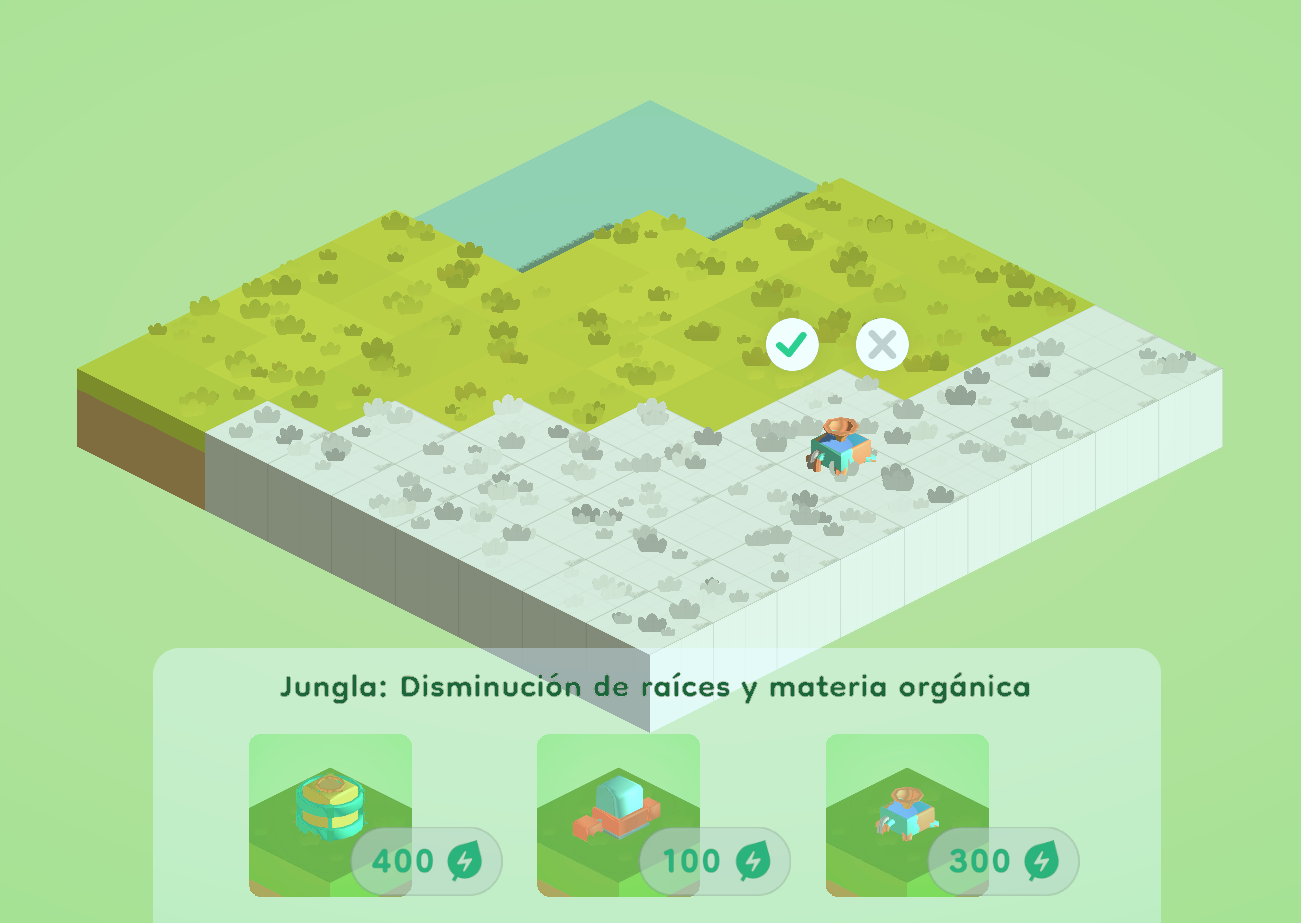
\includegraphics[width=350px,clip=true]{rango_infinito.png}
    \caption{Máquina de rango infinito}
    \label{fig:rango_inf}
  \end{figure}

  \begin{figure}[H]
    \centering
      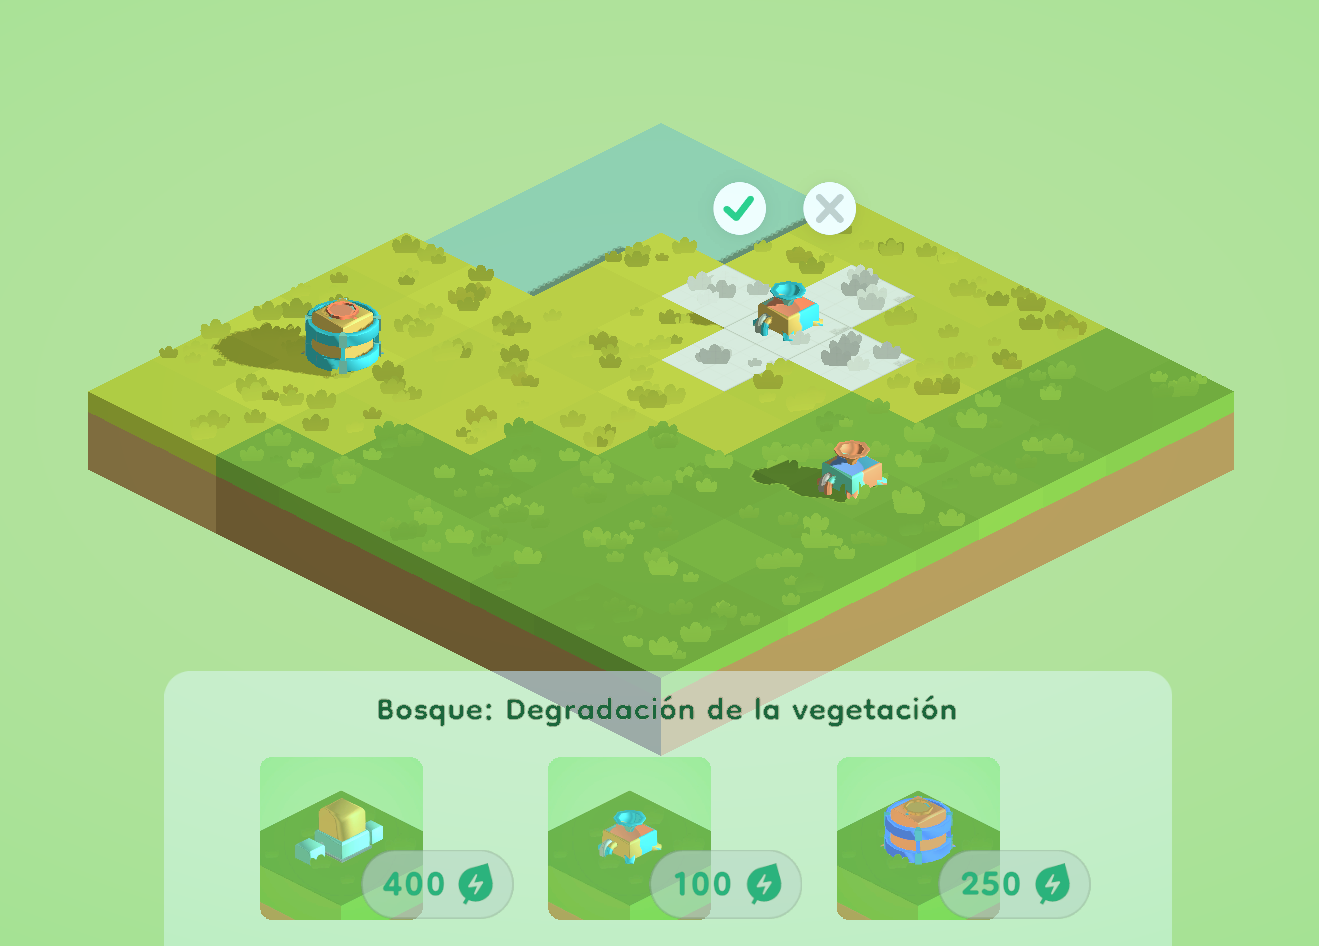
\includegraphics[width=350px,clip=true]{rango_chiquito.png}
    \caption{Máquina de rango por forma}
    \label{fig:rango_form}
  \end{figure}

La implementación de las máquinas con rango por forma es destacable dado que se utiliza una textura en blanco y negro (Figura \ref{fig:rango_pattern}) con la forma del rango que se quiera utilizar y esta se cachea al inicializar la máquina (Código \ref{alg:matrizmachine}) (durante la carga del nivel) en forma de una matriz bidimensional de ceros y unos, donde los unos son las casillas sobre las que actúa la máquina.
Esta implementación es bastante eficiente y permite limpiar las casillas que no son afectadas por la máquina a la vez que resaltan las que si lo son sin necesidad de hacer pasadas extra.

\begin{figure}[H]
    \centering
      
\includegraphics[width=350px,clip=true]{Cross_MachinePattern.png}
    \caption{Ejemplo de textura usado para el rango de una máquina}
    \label{fig:rango_pattern}
  \end{figure}

\begin{mypython}[caption={Código para cachear la matríz del rango de una máquina.},label={alg:matrizmachine}]
private void PrecalcTexture() 
{
    if (_patternTexture == null) return;
    _textureMatrix = new int[_patternTexture.width, _patternTexture.height];
    Color[] pixels = _patternTexture.GetPixels();
    for (int i = 0; i < _patternTexture.width; i++) 
    {
        for (int j = 0; j < _patternTexture.height; j++) 
        {
            Color currentPixel = pixels[i + (j * _patternTexture.width)];
            _textureMatrix[i, j] = currentPixel == Color.white ? 1 : 0;
        }
    }
}
\end{mypython}

La tienda (Figura \ref{fig:tienda}), por otro lado, es una interfaz de Unity basada en AnKuchen\cite{AnKuchen} (Figura \ref{fig:tiendaUML}), como todas las interfaces del juego. La tienda permite al jugador ver la información destacable de una máquina a la hora de comprarla (Restricción y valores asociados, precio y porcentaje de compleción añadido si aplica). 

\begin{figure}[H]
\centering
    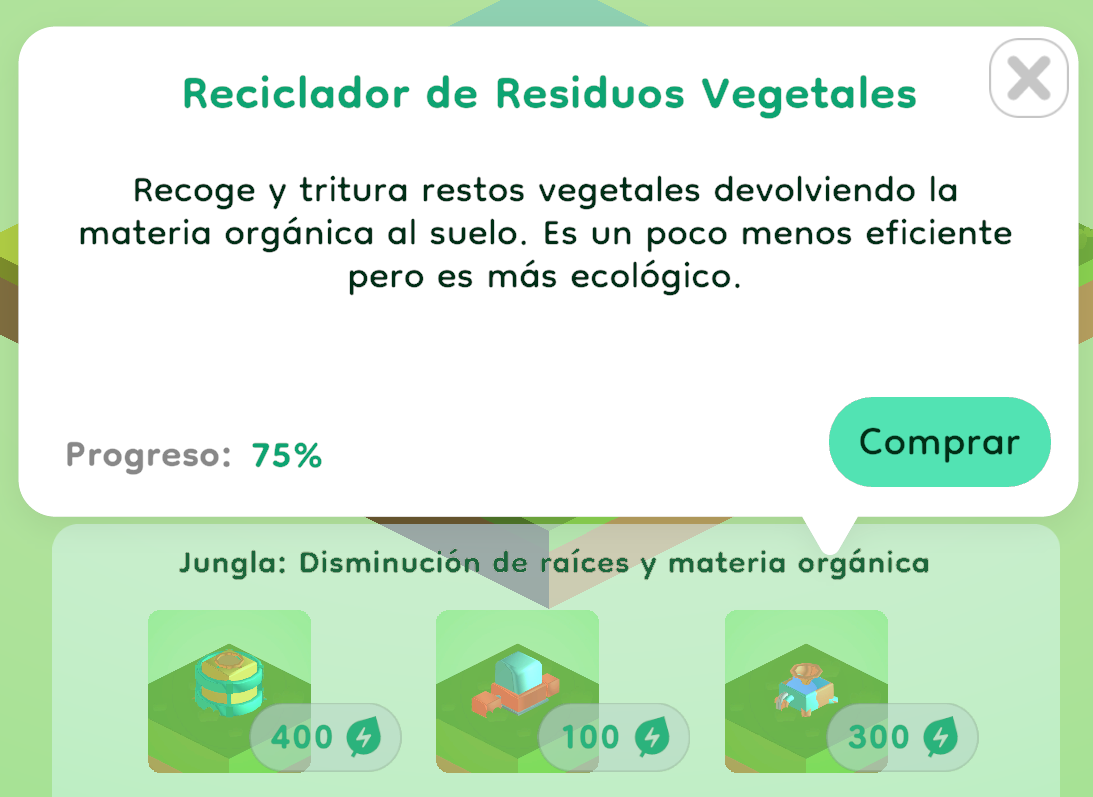
\includegraphics[width=350px,clip=true]{tienda.png}
\caption{Tienda de Máquinas, compra de una máquina que restaura el 75\% de una fase}
\label{fig:tienda}
\end{figure}

\begin{figure}[H]
\centering
    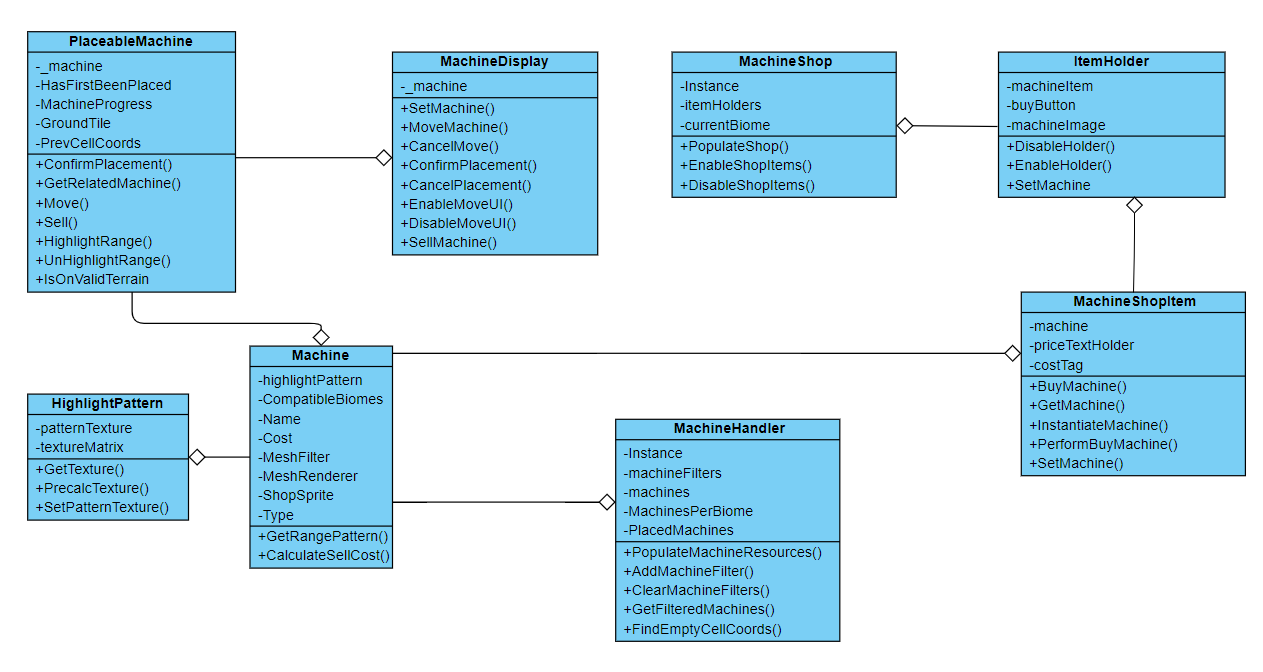
\includegraphics[width=350px,clip=true]{Machine_Shop_UI.png}
\caption{Diagrama de clases de la tienda}
\label{fig:tiendaUML}
\end{figure}

Al comprar una máquina desde la tienda se crea una instancia de un PlaceableMachine y se hace una copia profunda de la máquina asociada al 'ItemHolder' de la tienda. Esto permite obtener copias lógicas de las distintas máquinas utilizando un único prefab.


\subsection{Relaciones Visuales}

Una gran parte de EcoRescue es la fase de investigación, donde el jugador debe leer y relacionar los problemas de las alteraciones con otros problemas y sus respectivas consecuencias. La implementación de esto es una serie de rutinas que instancian un 'line renderer' por cada relación, y actualizan la posición del segundo punto del 'renderer' a la posición del cursor.

\begin{mypython}[caption={Código para dibujar la línea de relaciones.},label={alg:drawloop}]
private async UniTask DrawLoop(LineRenderer line) 
{
    await UniTask.Delay(0);
    
    if (!_performDraw) 
    {
        HandleMouseUp(line, GetScreenMousePos());
        return;
    }
    Vector3 mousePos = GetMousePositionWorldPos();
    Vector3 anchorPos = GetAnchorWorldPos();
    line.positionCount = 2;
    line.SetPosition(0, anchorPos);
    line.SetPosition(1, mousePos);
    DrawLoop(line).Forget();
}
\end{mypython}

\subsection{Desarrollo Multiplataforma}

EcoRescue es un videojuego multiplataforma, desarrollado para PC y Android, el desarrollo para que sea usable en ambas plataformas no ha sido muy complejo dado que el control en PC está mayormente basado en el uso de teclado y ratón.

La mayor parte del esfuerzo ha sido sobre todo en el escalado de la UI para que sea responsive, pero gracias a la implementación de Canvas\cite{unitycanvas} de Unity, se puede configurar la interfaz para que siempre respete el margen del lado en en la que esté colocado.

Otra parte del esfuerzo ha ido en la clase de ScreenSelector, que utiliza en Unity Input System\cite{unityinputsystem} para leer los eventos de touch o click y lo utiliza para intentar obtener los objetos de tipo selectable que haya en esas coordenadas del ratón pasadas a coordenadas del mundo virtual. Si el script encuentra un selectable en esas coordenadas que está habilitado, lanza el callback de OnClick.

La única adición relevante para soportar el desarrollo multiplataforma en este caso ha sido tener que diferenciar si la acción la está realizando un touch device (Código \ref{alg:selecttouch}) o un pointer al uso (Código \ref{alg:selectPC}).

\begin{mypython}[caption={Código para seleccionar una entidad en un 'Touch Device'.},label={alg:selecttouch}]
Touch touch;
touch = Input.GetTouch(0);
selectionRay = _camera.ScreenPointToRay(touch.position);
if (Physics.Raycast(selectionRay, out hit, _range, _selectableLayers) && touch.phase == UnityEngine.TouchPhase.Began)
{
    if (!EventSystem.current.IsPointerOverGameObject(touch.fingerId))
    {
        if (_selectedObject == null || _selectedObject.gameObject != hit.collider.gameObject)
        {
            TryToSelectTouch(hit.collider.gameObject, touch);
        }
        ConfirmTouch();
    }
}
else if (touch.phase == UnityEngine.TouchPhase.Canceled)
{
    if (_selectedObject)
    {
        _selectedObject.Deselect();
        _selectedObject = null;
        onNothingSelectedCallback?.Invoke();
    }
}
\end{mypython}

\begin{mypython}[caption={Código para seleccionar una entidad en PC.},label={alg:selectPC}]
selectionRay = _camera.ScreenPointToRay(Mouse.current.position.ReadValue());
if (Physics.Raycast(selectionRay, out hit, _range))
{
    if (EventSystem.current != null)
    {
        if (!EventSystem.current.IsPointerOverGameObject())
        {
            if (_selectedObject == null || _selectedObject.gameObject != hit.collider.gameObject)
            {
                TryToSelect(hit.collider.gameObject);
            }
            CheckClick();
        }
    }
}
else
{
    if (_selectedObject)
    {
        _selectedObject.Deselect();
        _selectedObject = null;
        onNothingSelectedCallback?.Invoke();
    }
}
\end{mypython}

\subsection{Telemetría}

De cara a la validación, se ha considerado importante que, aparte de hacer un cuestionario a los alumnos de 1º de la ESO que han validado el videojuego, era necesario recabar información en relación a las partidas que jueguen. 

Con este objetivo se ha utilizado la clase DBConnection que se encarga de hacer una conexión mediante un UnityWebRequest con MariaDB cada par de minutos y hace una subida a la base de datos con información sobre el jugador y la partida (Código \ref{alg:bbdd}), de cara a obtener la mayor cantidad de datos posible.
\begin{mypython}[caption={Código para hacer inserciones en la BBDD.},label={alg:bbdd}]
public void InsertUser(int id, string username, int age, 
    string gender, int machines_placed, int machines_sold, 
    int phase_success, int phase_fail, int duration, 
    int completion, Action<int> callback)
{
    string data = \$\@"{{
                    ""username"":""TFGMVAB"", 
                    ""password"":""2024TFGjuegogestionecoPC"", 
                    ""token"":""{token}"",
                    ""table"":""users"",
                    ""data"": {
                     {""user_id"":""{id}"",
                     ""name"": ""{username}"",
                     ""age"": ""{age}"",
                     ""gender"": ""{gender}"",
                     ""machines_placed"":""{machines_placed}"",
                     ""machines_sold"" : ""{machines_sold}"",
                     ""progress"" : ""{completion}"",
                     ""success_phase"" : ""{phase_success}"",
                     ""failure_phase"" : ""{phase_fail}"",
                     ""duration"" : ""{duration}""}}
    }}";
    Debug.Log(data);
    StartCoroutine(DBAccess(data, _insert, (request) =>
    {
        if (request.result != UnityWebRequest.Result.Success)
        {
            Debug.Log(request.downloadHandler.data);
        }
        else
        {
            // La solicitud fue exitosa, puedes acceder a la respuesta
            Debug.Log(request.downloadHandler.text);
        }
        request.Dispose();
    }));
}
\end{mypython}

\subsection{Asset Importer}

Como se ha mencionado varias veces a lo largo del documento, debido al enfoque procedimental del videojuego, ha sido necesario generar un enorme volumen de datos, por desgracia, al momento de generar una cantidad similar de ScriptableObjects se pudo ver que claramente eso generaría un cuello de botella abismal en el 'workflow'. Esto provocó que se tuviera que desarrollar un 'Asset Importer' que permitiese la generación automática de los ScriptableObjects necesarios para poblar el juego con el contenido deseado.

Este 'Asset Importer' tiene dos fases:
\begin{compactitem}
    \item Generación automática de Enumerados
    \item Generación automática de ScriptableObjects
\end{compactitem}

Cada fase tiene su propio MenuItem en la barra de tareas de unity y ambas generaciones leen los archivos en formato .csv encontrados en el directorio \textunderscore Data. 

La primera fase:
\begin{enumerate}
    \item Elimina los enumerados que se encuentran en la ruta Resources
    \item Itera todos y cada uno de los archivos csv y añade todas las ocurrencias únicas de ese enumerado a un diccionario.
    \item Imprime la lista sobre un buffer de bytes.
    \item Rellena un archivo en blanco con ese buffer.
\end{enumerate} 

De esta forma generamos código programáticamente para mantener siempe actualizado el listado de enumerados (Código \ref{alg:enviroenum}).

\begin{mypython}[caption={Código para autogenerar el enumerado de EnviroConsequences.},label={alg:enviroenum}]
static string RawConsequencesEnum(string[] lines)
{
    var output = "public enum EnviroConsequenceType{";
    foreach (var consequence in lines)
    {
        if (string.IsNullOrEmpty(consequence))
        {
            continue;
        }
        var tags = consequence.Split("|");
        output += GetTypeTagName(tags[3].Trim()) + ", ";
    }
    output += "}";
    return output;
}
\end{mypython}

La segunda fase:
\begin{enumerate}
    \item Itera por cada linea de cada archivo .csv.
    \item Genera una instancia de tipo 'Type' DTO (Data Transfer Object).
    \item Añade esa instancia a un diccionario que relaciona cada enumerado con su respectivo DTO (Código \ref{alg:enviroSO1}). 
    \item Una vez iteradas todas las líneas, se iteran todos las claves del diccionario.
    \item Por cada clave se crea un ScriptableObject de su respectivo tipo, y se hace una copia profunda de datos desde el DTO (Código \ref{alg:enviroSO2}) al ScriptableObject recién generado.
\end{enumerate} 

\begin{mypython}[caption={Código para autogenerar DTOs de tipo EnviroConsequences.},label={alg:enviroSO1}]
static Dictionary<EnviroConsequenceType, EnviroConsequence.EnviroConsequenceDTO> ParseConsequenceDict()
{
    var dict = new Dictionary<EnviroConsequenceType, EnviroConsequence.EnviroConsequenceDTO>();
    var lines = ConsequenceString();
    foreach (var line in lines)
    {
        if (string.IsNullOrEmpty(line))
            continue;
        var tags = line.Split("|");
        var dto = new EnviroConsequence.EnviroConsequenceDTO();
        dto.name = tags[0].Trim();
        dto.Title = tags[1].Trim();
        dto.Description = tags[2].Trim();
        dto.Type = (EnviroConsequenceType) Enum.Parse(typeof(EnviroConsequenceType), tags[3].Trim());
        dto.Sprite = FindSprite(tags[4].Trim());
        dto.color = GetColor(tags[5].Trim());
        dict[dto.Type] = dto;
    }
    return dict;
}
\end{mypython}

\begin{mypython}[caption={Código para autogenerar ScriptableObject de tipo EnviroConsequences.},label={alg:enviroSO2}]
static Dictionary<EnviroConsequenceType, EnviroConsequence> CreateConsequences()
{
    var consequences = new Dictionary<EnviroConsequenceType, EnviroConsequence>();
    var consequenceArray = Resources.LoadAll("ScriptableObjects/Consequences", typeof(EnviroConsequence));
    foreach (var consequence in consequenceArray.Cast<EnviroConsequence>())
    {
        consequences[consequence.Type] = consequence;
    }
    var consequenceDTODict = ParseConsequenceDict();
    foreach (var type in (EnviroConsequenceType[])System.Enum.GetValues(typeof(EnviroConsequenceType)))
    {
        if (!consequences.ContainsKey(type))
        {
            var newConsequence = ScriptableObject.CreateInstance<EnviroConsequence>();
            string assetPath = ImportMarroneroPath + "ScriptableObjects/" + "Consequences" + "/" + type.ToString() + ".asset";
            newConsequence.name = consequenceDTODict[type].name;
            newConsequence.Title = consequenceDTODict[type].Title;
            newConsequence.Description = consequenceDTODict[type].Description;
            newConsequence.Type = consequenceDTODict[type].Type;
            newConsequence.Sprite = consequenceDTODict[type].Sprite;
            newConsequence.color = consequenceDTODict[type].color;
            AssetDatabase.CreateAsset(newConsequence, assetPath);
            EditorUtility.SetDirty(newConsequence);
            AssetDatabase.SaveAssets();
            AssetDatabase.Refresh();
            EditorUtility.FocusProjectWindow();
            Selection.activeObject = newConsequence;
            consequences[type] = newConsequence;
        }
    }
    return consequences;
}
\end{mypython}

\subsection{AutoSlicer}

Se ha desarrollado también una pequeña herramienta usando el plugin Auto9Slicer\cite{Auto9Slicer} de kyubuns que permite hacer 'slice' automáticamente de sprites en formato png (Código \ref{alg:spriteslicer}), de forma que se puedan estirar sin deformarse. 

\begin{mypython}[caption={Código para aplicar automáticamente el algoritmo de slice sobre los sprites deseados.},label={alg:spriteslicer}]
[CustomEditor(typeof(Auto9SliceTester))]
public class Auto9SliceTesterEditor : Editor
{
    public override void OnInspectorGUI()
    {
        base.OnInspectorGUI();
        EditorGUILayout.Space(20);
        if (GUILayout.Button("Run")) ((Auto9SliceTester) target).Run();
    }
}

[CreateAssetMenu(menuName = "Auto 9Slice/Tester", fileName = nameof(Auto9SliceTester))]
public class Auto9SliceTester : ScriptableObject
{
    public SliceOptions Options => options;
    [SerializeField] private SliceOptions options = new SliceOptions();
    public bool CreateBackup => createBackup;
    [SerializeField] private bool createBackup = true;
    public void Run()
    {
        var directoryPath = Path.GetDirectoryName(AssetDatabase.GetAssetPath(this));
        if (directoryPath == null) throw new Exception(\$"directoryPath == null");
        var fullDirectoryPath = Path.Combine(Path.GetDirectoryName(Application.dataPath) ?? "", directoryPath);
        var targets = Directory.GetFiles(fullDirectoryPath)
            .Select(Path.GetFileName)
            .Where(x => x.EndsWith(".png") || x.EndsWith(".jpg") || x.EndsWith(".jpeg"))
            .Where(x => !x.Contains(".original"))
            .Select(x => Path.Combine(directoryPath, x))
            .Select(x => (Path: x, Texture: AssetDatabase.LoadAssetAtPath<Texture2D>(x)))
            .Where(x => x.Item2 != null)
            .ToArray();
        foreach (var target in targets)
        {
            var importer = AssetImporter.GetAtPath(target.Path);
            if (importer is TextureImporter textureImporter)
            {
                if (textureImporter.spriteBorder != Vector4.zero) continue;
                var fullPath = Path.Combine(Path.GetDirectoryName(Application.dataPath) ?? "", target.Path);
                var bytes = File.ReadAllBytes(fullPath);
                if (CreateBackup)
                {
                    var fileName = Path.GetFileNameWithoutExtension(fullPath);
                    File.WriteAllBytes(Path.Combine(Path.GetDirectoryName(fullPath) ?? "", fileName + ".original" + Path.GetExtension(fullPath)), bytes);
                }
                var targetTexture = new Texture2D(2, 2);
                targetTexture.LoadImage(bytes);
                var slicedTexture = Slicer.Slice(targetTexture, Options);
                textureImporter.textureType = TextureImporterType.Sprite;
                textureImporter.spriteBorder = slicedTexture.Border.ToVector4();
                if (fullPath.EndsWith(".png")) File.WriteAllBytes(fullPath, slicedTexture.Texture.EncodeToPNG());
                if (fullPath.EndsWith(".jpg")) File.WriteAllBytes(fullPath, slicedTexture.Texture.EncodeToJPG());
                if (fullPath.EndsWith(".jpeg")) File.WriteAllBytes(fullPath, slicedTexture.Texture.EncodeToJPG());
                Debug.Log(\$"Auto 9Slice {Path.GetFileName(target.Path)} = {textureImporter.spriteBorder}");
            }
        }
        AssetDatabase.Refresh();
    }
}
\end{mypython}